\subsection{Arquitetura da Malha Descentralizada}
\label{sub:arquitetura}

A arquitetura do HormuzNet foi projetada como uma malha (\textit{mesh}) autônoma de três camadas, conforme ilustra a Figura~\ref{fig:arquitetura}. A camada de aquisição utiliza sensores que publicam alertas em um endereço de \textit{UDP Multicast}. A camada de controle é composta por nove \textit{brokers} distribuídos geograficamente (B1 a B9 correspondendo a Noroeste, Norte, Nordeste, Leste, Sudeste, Sul, Sudoeste, Oeste e Centro/Líder de Descoberta), que formam uma rede P2P estável em malha cooperativa. A camada de atuação consiste em sete drones autônomos que gerenciam conexões TCP persistentes com a malha.

\begin{figure}[ht]
  \centering
  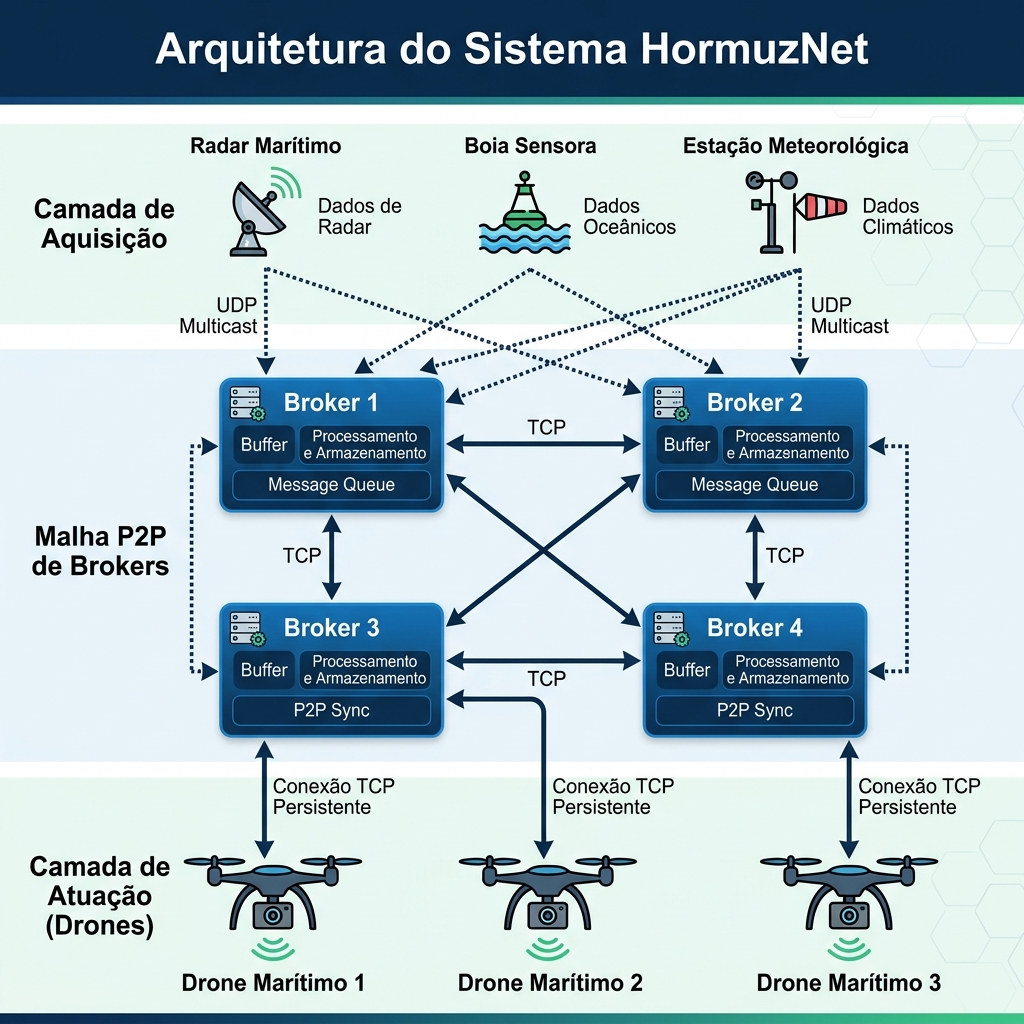
\includegraphics[width=0.88\textwidth]{figuras/arquitetura.png}
  \caption{Arquitetura descentralizada do HormuzNet: malha P2P entre brokers e descoberta de novos nós. Fonte: próprio autor.}
  \label{fig:arquitetura}
\end{figure}

\subsection{Componentes e Organização do Sistema}

O sistema é organizado em módulos independentes implementados em Go. Os principais componentes são:
\begin{itemize}
    \item \textbf{Broker:} Gerencia o estado global, sincroniza eventos via Lamport, executa a herança em anel (Ring Failover) de setores órfãos e coordena o despacho de drones.
    \item \textbf{Sensor:} Simula dispositivos ambientais que detectam ocorrências e as propagam via Multicast.
    \item \textbf{Drone:} Agente autônomo de resposta com lógica de \textit{fallback} e modelo de falha probabilístico.
    \item \textbf{Monitor:} Dashboard tático que consolida a visão da malha via WebSockets com lógica de de-duplicação de eventos.
\end{itemize}

\subsection{Protocolos de Rede e Justificativas}

A escolha dos protocolos seguiu critérios de resiliência e eficiência para cada perfil de tráfego:
\begin{itemize}
    \item \textbf{UDP Multicast (Porta 9876, endereço 224.1.2.3):} Utilizado para telemetria de sensores. A justificativa reside na necessidade de redundância: ao publicar em um grupo \textit{multicast}, o sensor garante que todos os \textit{brokers} ativos capturem o alerta sem precisar conhecer o IP de cada um.
    \item \textbf{TCP P2P e Drone-Broker (Portas 6000-6008):} Os \textit{brokers} mantêm conexões TCP diretas entre si para a propagação de relógios de Lamport, heartbeats e mensagens de coordenação. A mesma porta é compartilhada para o registro e controle de drones, otimizando o uso de sockets do sistema. O TCP garante a entrega confiável de mensagens de sincronização.
\end{itemize}

\subsection{Implementação da Concorrência}

A concorrência é o cerne do \textit{broker}, que precisa lidar simultaneamente com a rede P2P, os sensores e os drones. O uso de \textit{goroutines} permite que cada conexão seja tratada em um fio de execução independente. Para garantir a segurança de memória ao acessar a fila de ocorrências compartilhada, utilizou-se \textit{mutexes}. Abaixo, um trecho de código ilustra o processamento concorrente de mensagens Lamport:

\begin{verbatim}
func (b *Broker) handleP2PConnection(conn net.Conn) {
    defer conn.Close()
    decoder := json.NewDecoder(conn)
    for {
        var msg P2PMessage
        if err := decoder.Decode(&msg); err != nil { break }
        
        b.mu.Lock()
        // Sincronização do Relógio de Lamport
        if msg.Timestamp > b.lamportClock {
            b.lamportClock = msg.Timestamp
        }
        b.lamportClock++
        b.mu.Unlock()
        
        b.processEvent(msg)
    }
}
\end{verbatim}

\subsection{Decisões de Design e Resiliência}

Uma decisão crítica foi o modelo de \textit{fallback} dos drones. Caso um \textit{broker} falhe, o drone tenta reconexão com o próximo \textit{broker} da lista configurada. Além disso, implementou-se a exclusão mútua distribuída baseada na ordem de Lamport: todos os \textit{brokers} enxergam a mesma fila, mas apenas o \textit{broker} que possui a conexão ativa com o drone mais próximo executa o despacho, notificando os demais para removerem a ocorrência da fila.

Outra decisão importante foi a inclusão de um modelo de falha realístico: drones possuem 10\% de chance de serem "abatidos" durante uma missão. Esta lógica força o sistema a tratar a perda de agentes de atuação e reatribuir missões, testando a robustez da malha sob condições adversas.

Para garantir a estabilidade do sistema sob o modelo de falhas com alta taxa de recomposição (onde drones redefinem conexões rapidamente após abates), foi implementada uma proteção contra condições de corrida nas conexões TCP persistentes. Nos blocos de encerramento (\textit{defer}) dos loops de leitura de drones e de brokers vizinhos, a remoção do nó correspondente dos mapas ativos do sistema é realizada apenas se a conexão que está sendo fechada corresponder exatamente à conexão registrada no mapa. Caso um nó se reconecte sob uma nova conexão antes do encerramento da goroutine da conexão anterior, a remoção e marcação de indisponibilidade é ignorada para a conexão antiga, impedindo que o nó ativo seja indevidamente desvinculado ou marcado como offline.

